\documentclass[12pt,a4paper]{article}
\usepackage[utf8]{vietnam}
\usepackage{amsmath,amssymb}
\usepackage{tabularx}
\usepackage{tikz}
\usepackage{xcolor}
\usepackage[top=0.6cm, bottom=0.6cm, left=0.6cm, right=0.6cm]{geometry}
\usepackage[dethi]{ex_test}

\SAOPTN{widthSA=2.6,heightSA=0.62}
\setlength{\parskip}{0pt}

% Dong ke cham mo chuan viet tay
\newcommand{\dongke}[1]{%
  \begingroup%
  \setlength{\parskip}{0pt}%
  \baselineskip=18.5pt%
  \vspace{1.0mm}%
  \foreach \i in {1,...,#1}{%
    \noindent{\color{gray!60}\dotfill}\par%
  }%
  \vspace{0.6mm}%
  \endgroup%
}

% Dinh nghia o bai tap tu luan trong bang
\newcommand{\oBaiTap}[3][5]{%
  \vspace{1.0mm}%
  \noindent\textbf{#2} #3\par%
  \dongke{#1}%
}

\begin{document}
\pagestyle{empty}
% =============================================================================
% ========================= TOAN 9 TUAN 11 BUOI 01 - MA DE 101 =================
% ========================= TRANG 1/2 ==========================================
% =============================================================================
\noindent
\begin{tabularx}{\linewidth}{|X|c|}
\hline
\textbf{PHIẾU KIỂM TRA ĐỊNH KỲ TOÁN 9 - TUẦN 11 - BUỔI 01} & \textbf{Mã đề: 101 - Trang 1/2} \\
\hline
\end{tabularx}

\vspace{1.0mm}

\noindent
\begin{tabularx}{\linewidth}{|p{3.2cm}|X|}
\hline
\centering\textbf{ĐIỂM SỐ} & \centering\textbf{LỜI NHẬN XÉT CỦA THẦY CÔ} \tabularnewline
\hline
\rule{0pt}{1.8cm} & \tabularnewline
\hline
\end{tabularx}

\vspace{1.2mm}
\noindent\textbf{Câu 1 (0,25 điểm).} Cho $(O; 6\text{ cm})$, cung tròn có số đo $60^\circ$. Độ dài cung là: \shortans{2\pi\text{ cm}}\par\vspace{0.6mm}
\noindent\textbf{Câu 2 (0,25 điểm).} Đường tròn có chu vi $C = 16\pi\text{ cm}$. Bán kính $R$ bằng: \shortans{8\text{ cm}}\par\vspace{0.6mm}
\noindent\textbf{Câu 3 (0,25 điểm).} Cho $(O; 12\text{ cm})$ có cung độ dài $3\pi\text{ cm}$. Số đo cung là: \shortans{45^\circ}\par\vspace{0.6mm}
\noindent\textbf{Câu 4 (0,25 điểm).} Căn bậc hai số học của $144$ là: \shortans{12}\par\vspace{0.6mm}
\noindent\textbf{Câu 5 (0,25 điểm).} Điều kiện xác định của biểu thức $\sqrt{2x - 8}$ là: \shortans{x \ge 4}\par\vspace{0.6mm}
\noindent\textbf{Câu 6 (0,25 điểm).} Tính giá trị của biểu thức $\sqrt{50} - \sqrt{18} + \sqrt{8} = $ \shortans{4\sqrt{2}}\par\vspace{0.6mm}
\noindent\textbf{Câu 7 (0,25 điểm).} Hệ phương trình $\begin{cases} 3x - y = 7 \\ x + y = 5 \end{cases}$ có nghiệm $(x; y)$ là: \shortans{(3; 2)}\par\vspace{0.6mm}
\noindent\textbf{Câu 8 (0,25 điểm).} Tam giác vuông có hai cạnh góc vuông $6\text{ cm}, 8\text{ cm}$. Đường cao là: \shortans{4{,}8\text{ cm}}\par\vspace{0.6mm}
\noindent\textbf{Câu 9 (0,25 điểm).} Tiếp tuyến của $(O)$ vuông góc với bán kính đi qua điểm nào: \shortans{\text{tiếp điểm}}\par\vspace{0.6mm}
\noindent\textbf{Câu 10 (0,25 điểm).} Bánh xe có đường kính $60\text{ cm}$, khi lăn $10$ vòng đi được: \shortans{6\pi\text{ m}}\par\vspace{0.6mm}
\vspace{0.6mm}
\noindent\textbf{Câu 11 (2,5 điểm).}
\vspace{0.6mm}

\noindent
\begin{tabularx}{\linewidth}{|X|X|}
\hline
\oBaiTap[20]{a) (1,25 điểm)}{Giải hệ phương trình:\par $\begin{cases} 2x - 3y = 1 \\ 3x + 2y = 8 \end{cases}$} & 
\oBaiTap[20]{b) (1,25 điểm)}{Cho biểu thức $P = \left(\dfrac{\sqrt{x}}{\sqrt{x} + 2} + \dfrac{4\sqrt{x}}{x - 4}\right) : \dfrac{\sqrt{x} + 2}{x - 4}$ với $x \ge 0, x \ne 4$.\par Rút gọn $P$ và tính giá trị của $P$ tại $x = 9$.} \\
\hline
\end{tabularx}

\newpage
% =============================================================================
% ========================= TOAN 9 TUAN 11 BUOI 01 - MA DE 101 =================
% ========================= TRANG 2/2 ==========================================
% =============================================================================
\noindent
\begin{tabularx}{\linewidth}{|X|c|}
\hline
\textbf{TOÁN 9 - TUẦN 11 - BUỔI 01} & \textbf{Mã đề: 101 - Trang 2/2} \\
\hline
\end{tabularx}

\vspace{1.5mm}

\noindent
\begin{tabularx}{\linewidth}{|X|}
\hline
\vspace{0.5mm}
\textbf{Câu 12 (2,5 điểm).} Hai tổ công nhân cùng làm chung một công việc thì hoàn thành trong $12$ giờ. Nếu tổ I làm trong $4$ giờ rồi nghỉ, tổ II làm tiếp trong $9$ giờ thì cả hai tổ hoàn thành được $\dfrac{7}{12}$ công việc. Hỏi nếu làm riêng thì mỗi tổ hoàn thành công việc đó trong bao lâu?\par
\vspace{0.4mm}
\noindent\textit{Bài giải:}\dongke{15}
\\ \hline
\end{tabularx}

\vspace{3.5mm}

\noindent
\begin{tabularx}{\linewidth}{|X|}
\hline
\vspace{0.5mm}
\begin{minipage}[t]{0.68\linewidth}
\vspace{0pt}
\textbf{Câu 13 (2,5 điểm).} Cho đường tròn $(O; R)$ và điểm $A$ nằm bên ngoài đường tròn. Từ $A$ kẻ hai tiếp tuyến $AB, AC$ với $(O)$ ($B, C$ là các tiếp điểm). Gọi $H$ là giao điểm của $OA$ và $BC$.\par\vspace{0.4mm}
\textbf{a) (1,25 điểm)} Chứng minh $OA \perp BC$ tại $H$. Cho $R = 6\text{ cm}$ và $\widehat{BOC} = 120^\circ$, hãy tính độ dài cung nhỏ $\wideparen{BC}$ của $(O)$.\par\vspace{0.4mm}
\textbf{b) (1,25 điểm)} Kẻ đường kính $BD$ của đường tròn $(O)$. Chứng minh $CD \parallel OA$.
\end{minipage}\hfill
\begin{minipage}[t]{0.30\linewidth}
\vspace{0pt}\centering
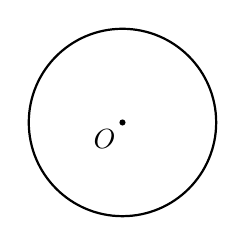
\begin{tikzpicture}[scale=0.85, >=stealth, line join=round, line cap=round]
  \coordinate (O) at (0, 0);
  \draw[thick] (O) circle (1.4cm);
  \fill (O) circle (1.3pt) node[below left=-1pt] {$O$};
\end{tikzpicture}
\end{minipage}\par
\vspace{0.4mm}
\noindent\textit{Bài giải:}\dongke{15}
\\ \hline
\end{tabularx}

\newpage
% =============================================================================
% ========================= TOAN 9 TUAN 11 BUOI 01 - MA DE 102 =================
% ========================= TRANG 1/2 ==========================================
% =============================================================================
\noindent
\begin{tabularx}{\linewidth}{|X|c|}
\hline
\textbf{PHIẾU KIỂM TRA ĐỊNH KỲ TOÁN 9 - TUẦN 11 - BUỔI 01} & \textbf{Mã đề: 102 - Trang 1/2} \\
\hline
\end{tabularx}

\vspace{1.0mm}

\noindent
\begin{tabularx}{\linewidth}{|p{3.2cm}|X|}
\hline
\centering\textbf{ĐIỂM SỐ} & \centering\textbf{LỜI NHẬN XÉT CỦA THẦY CÔ} \tabularnewline
\hline
\rule{0pt}{1.8cm} & \tabularnewline
\hline
\end{tabularx}

\vspace{1.2mm}
\noindent\textbf{Câu 1 (0,25 điểm).} Cho $(O; 9\text{ cm})$, cung tròn có số đo $40^\circ$. Độ dài cung là: \shortans{2\pi\text{ cm}}\par\vspace{0.6mm}
\noindent\textbf{Câu 2 (0,25 điểm).} Đường tròn có chu vi $C = 18\pi\text{ cm}$. Bán kính $R$ bằng: \shortans{9\text{ cm}}\par\vspace{0.6mm}
\noindent\textbf{Câu 3 (0,25 điểm).} Cho $(O; 10\text{ cm})$ có cung độ dài $5\pi\text{ cm}$. Số đo cung là: \shortans{90^\circ}\par\vspace{0.6mm}
\noindent\textbf{Câu 4 (0,25 điểm).} Căn bậc hai số học của $169$ là: \shortans{13}\par\vspace{0.6mm}
\noindent\textbf{Câu 5 (0,25 điểm).} Điều kiện xác định của biểu thức $\sqrt{3x - 12}$ là: \shortans{x \ge 4}\par\vspace{0.6mm}
\noindent\textbf{Câu 6 (0,25 điểm).} Tính giá trị của biểu thức $\sqrt{75} - \sqrt{27} + \sqrt{12} = $ \shortans{4\sqrt{3}}\par\vspace{0.6mm}
\noindent\textbf{Câu 7 (0,25 điểm).} Hệ phương trình $\begin{cases} 2x - y = 5 \\ x + y = 4 \end{cases}$ có nghiệm $(x; y)$ là: \shortans{(3; 1)}\par\vspace{0.6mm}
\noindent\textbf{Câu 8 (0,25 điểm).} Tam giác vuông có hai cạnh góc vuông $9\text{ cm}, 12\text{ cm}$. Đường cao là: \shortans{7{,}2\text{ cm}}\par\vspace{0.6mm}
\noindent\textbf{Câu 9 (0,25 điểm).} Đường thẳng vuông góc bán kính tại điểm trên đường tròn là: \shortans{\text{tiếp tuyến}}\par\vspace{0.6mm}
\noindent\textbf{Câu 10 (0,25 điểm).} Bánh xe có đường kính $70\text{ cm}$, khi lăn $10$ vòng đi được: \shortans{7\pi\text{ m}}\par\vspace{0.6mm}
\vspace{0.6mm}
\noindent\textbf{Câu 11 (2,5 điểm).}
\vspace{0.6mm}

\noindent
\begin{tabularx}{\linewidth}{|X|X|}
\hline
\oBaiTap[20]{a) (1,25 điểm)}{Giải hệ phương trình:\par $\begin{cases} 3x + 2y = 7 \\ 2x - 3y = -4 \end{cases}$} & 
\oBaiTap[20]{b) (1,25 điểm)}{Cho biểu thức $P = \left(\dfrac{\sqrt{x}}{\sqrt{x} + 3} + \dfrac{6\sqrt{x}}{x - 9}\right) : \dfrac{\sqrt{x} + 3}{x - 9}$ với $x \ge 0, x \ne 9$.\par Rút gọn $P$ và tính giá trị của $P$ tại $x = 16$.} \\
\hline
\end{tabularx}

\newpage
% =============================================================================
% ========================= TOAN 9 TUAN 11 BUOI 01 - MA DE 102 =================
% ========================= TRANG 2/2 ==========================================
% =============================================================================
\noindent
\begin{tabularx}{\linewidth}{|X|c|}
\hline
\textbf{TOÁN 9 - TUẦN 11 - BUỔI 01} & \textbf{Mã đề: 102 - Trang 2/2} \\
\hline
\end{tabularx}

\vspace{1.5mm}

\noindent
\begin{tabularx}{\linewidth}{|X|}
\hline
\vspace{0.5mm}
\textbf{Câu 12 (2,5 điểm).} Hai đội công nhân cùng sửa một đoạn đường thì hoàn thành trong $12$ ngày. Nếu đội I làm trong $3$ ngày rồi nghỉ, đội II làm tiếp trong $8$ ngày thì cả hai đội sửa được $\dfrac{1}{2}$ đoạn đường. Hỏi nếu làm riêng thì mỗi đội sửa xong đoạn đường trong bao lâu?\par
\vspace{0.4mm}
\noindent\textit{Bài giải:}\dongke{15}
\\ \hline
\end{tabularx}

\vspace{3.5mm}

\noindent
\begin{tabularx}{\linewidth}{|X|}
\hline
\vspace{0.5mm}
\begin{minipage}[t]{0.68\linewidth}
\vspace{0pt}
\textbf{Câu 13 (2,5 điểm).} Cho đường tròn $(O; R)$ và điểm $A$ nằm bên ngoài đường tròn. Từ $A$ kẻ hai tiếp tuyến $AB, AC$ với $(O)$ ($B, C$ là các tiếp điểm). Gọi $H$ là giao điểm của $OA$ và $BC$.\par\vspace{0.4mm}
\textbf{a) (1,25 điểm)} Chứng minh $OA \perp BC$ tại $H$. Cho $R = 9\text{ cm}$ và $\widehat{BOC} = 80^\circ$, hãy tính độ dài cung nhỏ $\wideparen{BC}$ của $(O)$.\par\vspace{0.4mm}
\textbf{b) (1,25 điểm)} Kẻ đường kính $BD$ của đường tròn $(O)$. Chứng minh $CD \parallel OA$.
\end{minipage}\hfill
\begin{minipage}[t]{0.30\linewidth}
\vspace{0pt}\centering
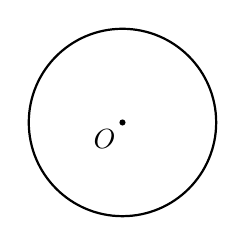
\begin{tikzpicture}[scale=0.85, >=stealth, line join=round, line cap=round]
  \coordinate (O) at (0, 0);
  \draw[thick] (O) circle (1.4cm);
  \fill (O) circle (1.3pt) node[below left=-1pt] {$O$};
\end{tikzpicture}
\end{minipage}\par
\vspace{0.4mm}
\noindent\textit{Bài giải:}\dongke{15}
\\ \hline
\end{tabularx}

\newpage
% =============================================================================
% ========================= TOAN 9 TUAN 11 BUOI 01 - MA DE 103 =================
% ========================= TRANG 1/2 ==========================================
% =============================================================================
\noindent
\begin{tabularx}{\linewidth}{|X|c|}
\hline
\textbf{PHIẾU KIỂM TRA ĐỊNH KỲ TOÁN 9 - TUẦN 11 - BUỔI 01} & \textbf{Mã đề: 103 - Trang 1/2} \\
\hline
\end{tabularx}

\vspace{1.0mm}

\noindent
\begin{tabularx}{\linewidth}{|p{3.2cm}|X|}
\hline
\centering\textbf{ĐIỂM SỐ} & \centering\textbf{LỜI NHẬN XÉT CỦA THẦY CÔ} \tabularnewline
\hline
\rule{0pt}{1.8cm} & \tabularnewline
\hline
\end{tabularx}

\vspace{1.2mm}
\noindent\textbf{Câu 1 (0,25 điểm).} Cho $(O; 4\text{ cm})$, cung tròn có số đo $90^\circ$. Độ dài cung là: \shortans{2\pi\text{ cm}}\par\vspace{0.6mm}
\noindent\textbf{Câu 2 (0,25 điểm).} Đường tròn có chu vi $C = 20\pi\text{ cm}$. Bán kính $R$ bằng: \shortans{10\text{ cm}}\par\vspace{0.6mm}
\noindent\textbf{Câu 3 (0,25 điểm).} Cho $(O; 18\text{ cm})$ có cung độ dài $6\pi\text{ cm}$. Số đo cung là: \shortans{60^\circ}\par\vspace{0.6mm}
\noindent\textbf{Câu 4 (0,25 điểm).} Căn bậc hai số học của $196$ là: \shortans{14}\par\vspace{0.6mm}
\noindent\textbf{Câu 5 (0,25 điểm).} Điều kiện xác định của biểu thức $\sqrt{5x - 15}$ là: \shortans{x \ge 3}\par\vspace{0.6mm}
\noindent\textbf{Câu 6 (0,25 điểm).} Tính giá trị của biểu thức $\sqrt{48} - \sqrt{12} + \sqrt{27} = $ \shortans{5\sqrt{3}}\par\vspace{0.6mm}
\noindent\textbf{Câu 7 (0,25 điểm).} Hệ phương trình $\begin{cases} 3x + y = 10 \\ x - y = 2 \end{cases}$ có nghiệm $(x; y)$ là: \shortans{(3; 1)}\par\vspace{0.6mm}
\noindent\textbf{Câu 8 (0,25 điểm).} Tam giác vuông có hai cạnh góc vuông $3\text{ cm}, 4\text{ cm}$. Đường cao là: \shortans{2{,}4\text{ cm}}\par\vspace{0.6mm}
\noindent\textbf{Câu 9 (0,25 điểm).} Số tiếp tuyến kẻ từ điểm ngoài đường tròn tới $(O)$ là: \shortans{2}\par\vspace{0.6mm}
\noindent\textbf{Câu 10 (0,25 điểm).} Bánh xe có đường kính $50\text{ cm}$, khi lăn $10$ vòng đi được: \shortans{5\pi\text{ m}}\par\vspace{0.6mm}
\vspace{0.6mm}
\noindent\textbf{Câu 11 (2,5 điểm).}
\vspace{0.6mm}

\noindent
\begin{tabularx}{\linewidth}{|X|X|}
\hline
\oBaiTap[20]{a) (1,25 điểm)}{Giải hệ phương trình:\par $\begin{cases} 3x - 2y = 4 \\ 2x + 3y = 7 \end{cases}$} & 
\oBaiTap[20]{b) (1,25 điểm)}{Cho biểu thức $P = \left(\dfrac{\sqrt{x}}{\sqrt{x} + 1} + \dfrac{2\sqrt{x}}{x - 1}\right) : \dfrac{\sqrt{x} + 1}{x - 1}$ với $x \ge 0, x \ne 1$.\par Rút gọn $P$ và tính giá trị của $P$ tại $x = 25$.} \\
\hline
\end{tabularx}

\newpage
% =============================================================================
% ========================= TOAN 9 TUAN 11 BUOI 01 - MA DE 103 =================
% ========================= TRANG 2/2 ==========================================
% =============================================================================
\noindent
\begin{tabularx}{\linewidth}{|X|c|}
\hline
\textbf{TOÁN 9 - TUẦN 11 - BUỔI 01} & \textbf{Mã đề: 103 - Trang 2/2} \\
\hline
\end{tabularx}

\vspace{1.5mm}

\noindent
\begin{tabularx}{\linewidth}{|X|}
\hline
\vspace{0.5mm}
\textbf{Câu 12 (2,5 điểm).} Hai vòi nước cùng chảy vào một bể cạn thì đầy bể sau $6$ giờ. Nếu mở vòi I chảy trong $2$ giờ rồi khóa lại và mở vòi II chảy tiếp trong $5$ giờ thì cả hai vòi chảy được $\dfrac{8}{15}$ bể nước. Hỏi nếu chảy riêng thì mỗi vòi chảy đầy bể trong bao lâu?\par
\vspace{0.4mm}
\noindent\textit{Bài giải:}\dongke{15}
\\ \hline
\end{tabularx}

\vspace{3.5mm}

\noindent
\begin{tabularx}{\linewidth}{|X|}
\hline
\vspace{0.5mm}
\begin{minipage}[t]{0.68\linewidth}
\vspace{0pt}
\textbf{Câu 13 (2,5 điểm).} Cho đường tròn $(O; R)$ và điểm $A$ nằm bên ngoài đường tròn. Từ $A$ kẻ hai tiếp tuyến $AB, AC$ với $(O)$ ($B, C$ là các tiếp điểm). Gọi $H$ là giao điểm của $OA$ và $BC$.\par\vspace{0.4mm}
\textbf{a) (1,25 điểm)} Chứng minh $OA \perp BC$ tại $H$. Cho $R = 8\text{ cm}$ và $\widehat{BOC} = 90^\circ$, hãy tính độ dài cung nhỏ $\wideparen{BC}$ của $(O)$.\par\vspace{0.4mm}
\textbf{b) (1,25 điểm)} Kẻ đường kính $BD$ của đường tròn $(O)$. Chứng minh $CD \parallel OA$.
\end{minipage}\hfill
\begin{minipage}[t]{0.30\linewidth}
\vspace{0pt}\centering
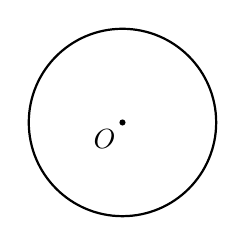
\begin{tikzpicture}[scale=0.85, >=stealth, line join=round, line cap=round]
  \coordinate (O) at (0, 0);
  \draw[thick] (O) circle (1.4cm);
  \fill (O) circle (1.3pt) node[below left=-1pt] {$O$};
\end{tikzpicture}
\end{minipage}\par
\vspace{0.4mm}
\noindent\textit{Bài giải:}\dongke{15}
\\ \hline
\end{tabularx}

\newpage
% =============================================================================
% ========================= TOAN 9 TUAN 11 BUOI 01 - MA DE 104 =================
% ========================= TRANG 1/2 ==========================================
% =============================================================================
\noindent
\begin{tabularx}{\linewidth}{|X|c|}
\hline
\textbf{PHIẾU KIỂM TRA ĐỊNH KỲ TOÁN 9 - TUẦN 11 - BUỔI 01} & \textbf{Mã đề: 104 - Trang 1/2} \\
\hline
\end{tabularx}

\vspace{1.0mm}

\noindent
\begin{tabularx}{\linewidth}{|p{3.2cm}|X|}
\hline
\centering\textbf{ĐIỂM SỐ} & \centering\textbf{LỜI NHẬN XÉT CỦA THẦY CÔ} \tabularnewline
\hline
\rule{0pt}{1.8cm} & \tabularnewline
\hline
\end{tabularx}

\vspace{1.2mm}
\noindent\textbf{Câu 1 (0,25 điểm).} Cho $(O; 10\text{ cm})$, cung tròn có số đo $36^\circ$. Độ dài cung là: \shortans{2\pi\text{ cm}}\par\vspace{0.6mm}
\noindent\textbf{Câu 2 (0,25 điểm).} Đường tròn có chu vi $C = 12\pi\text{ cm}$. Bán kính $R$ bằng: \shortans{6\text{ cm}}\par\vspace{0.6mm}
\noindent\textbf{Câu 3 (0,25 điểm).} Cho $(O; 15\text{ cm})$ có cung độ dài $2{,}5\pi\text{ cm}$. Số đo cung là: \shortans{30^\circ}\par\vspace{0.6mm}
\noindent\textbf{Câu 4 (0,25 điểm).} Căn bậc hai số học của $225$ là: \shortans{15}\par\vspace{0.6mm}
\noindent\textbf{Câu 5 (0,25 điểm).} Điều kiện xác định của biểu thức $\sqrt{4x - 20}$ là: \shortans{x \ge 5}\par\vspace{0.6mm}
\noindent\textbf{Câu 6 (0,25 điểm).} Tính giá trị của biểu thức $\sqrt{32} - \sqrt{8} + \sqrt{18} = $ \shortans{5\sqrt{2}}\par\vspace{0.6mm}
\noindent\textbf{Câu 7 (0,25 điểm).} Hệ phương trình $\begin{cases} 2x + y = 8 \\ x - y = 1 \end{cases}$ có nghiệm $(x; y)$ là: \shortans{(3; 2)}\par\vspace{0.6mm}
\noindent\textbf{Câu 8 (0,25 điểm).} Tam giác vuông có hai cạnh góc vuông $12\text{ cm}, 16\text{ cm}$. Đường cao là: \shortans{9{,}6\text{ cm}}\par\vspace{0.6mm}
\noindent\textbf{Câu 9 (0,25 điểm).} Khoảng cách từ tâm tới tiếp tuyến của $(O; R)$ là: \shortans{R}\par\vspace{0.6mm}
\noindent\textbf{Câu 10 (0,25 điểm).} Bánh xe có đường kính $80\text{ cm}$, khi lăn $10$ vòng đi được: \shortans{8\pi\text{ m}}\par\vspace{0.6mm}
\vspace{0.6mm}
\noindent\textbf{Câu 11 (2,5 điểm).}
\vspace{0.6mm}

\noindent
\begin{tabularx}{\linewidth}{|X|X|}
\hline
\oBaiTap[20]{a) (1,25 điểm)}{Giải hệ phương trình:\par $\begin{cases} 2x + 3y = 8 \\ 3x - 2y = -1 \end{cases}$} & 
\oBaiTap[20]{b) (1,25 điểm)}{Cho biểu thức $P = \left(\dfrac{\sqrt{x}}{\sqrt{x} + 4} + \dfrac{8\sqrt{x}}{x - 16}\right) : \dfrac{\sqrt{x} + 4}{x - 16}$ với $x \ge 0, x \ne 16$.\par Rút gọn $P$ và tính giá trị của $P$ tại $x = 4$.} \\
\hline
\end{tabularx}

\newpage
% =============================================================================
% ========================= TOAN 9 TUAN 11 BUOI 01 - MA DE 104 =================
% ========================= TRANG 2/2 ==========================================
% =============================================================================
\noindent
\begin{tabularx}{\linewidth}{|X|c|}
\hline
\textbf{TOÁN 9 - TUẦN 11 - BUỔI 01} & \textbf{Mã đề: 104 - Trang 2/2} \\
\hline
\end{tabularx}

\vspace{1.5mm}

\noindent
\begin{tabularx}{\linewidth}{|X|}
\hline
\vspace{0.5mm}
\textbf{Câu 12 (2,5 điểm).} Hai vòi nước cùng chảy vào một bể cạn thì đầy bể sau $4$ giờ. Nếu mở vòi I chảy trong $3$ giờ rồi khóa lại và mở vòi II chảy tiếp trong $2$ giờ thì cả hai vòi chảy được $\dfrac{2}{3}$ bể nước. Hỏi nếu chảy riêng thì mỗi vòi chảy đầy bể trong bao lâu?\par
\vspace{0.4mm}
\noindent\textit{Bài giải:}\dongke{15}
\\ \hline
\end{tabularx}

\vspace{3.5mm}

\noindent
\begin{tabularx}{\linewidth}{|X|}
\hline
\vspace{0.5mm}
\begin{minipage}[t]{0.68\linewidth}
\vspace{0pt}
\textbf{Câu 13 (2,5 điểm).} Cho đường tròn $(O; R)$ và điểm $A$ nằm bên ngoài đường tròn. Từ $A$ kẻ hai tiếp tuyến $AB, AC$ với $(O)$ ($B, C$ là các tiếp điểm). Gọi $H$ là giao điểm của $OA$ và $BC$.\par\vspace{0.4mm}
\textbf{a) (1,25 điểm)} Chứng minh $OA \perp BC$ tại $H$. Cho $R = 12\text{ cm}$ và $\widehat{BOC} = 60^\circ$, hãy tính độ dài cung nhỏ $\wideparen{BC}$ của $(O)$.\par\vspace{0.4mm}
\textbf{b) (1,25 điểm)} Kẻ đường kính $BD$ của đường tròn $(O)$. Chứng minh $CD \parallel OA$.
\end{minipage}\hfill
\begin{minipage}[t]{0.30\linewidth}
\vspace{0pt}\centering
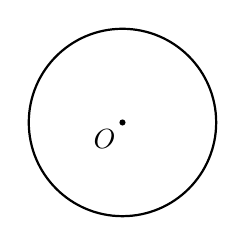
\begin{tikzpicture}[scale=0.85, >=stealth, line join=round, line cap=round]
  \coordinate (O) at (0, 0);
  \draw[thick] (O) circle (1.4cm);
  \fill (O) circle (1.3pt) node[below left=-1pt] {$O$};
\end{tikzpicture}
\end{minipage}\par
\vspace{0.4mm}
\noindent\textit{Bài giải:}\dongke{15}
\\ \hline
\end{tabularx}
\end{document}
